\documentclass[11pt]{article}
\usepackage[T1]{fontenc}
\usepackage{lmodern,microtype}
\usepackage[margin=1in]{geometry}
\usepackage{amsmath,amssymb,amsthm,mathtools}
\usepackage{graphicx,booktabs,array}
\usepackage{caption,enumitem}
\usepackage[numbers,sort&compress]{natbib}
\usepackage{xcolor,tikz}
\usetikzlibrary{arrows.meta,positioning}
\usepackage{placeins,xurl}
\usepackage[colorlinks=true,linkcolor=blue!45!black,citecolor=blue!45!black,urlcolor=blue!45!black]{hyperref}
\hypersetup{pdftitle={From samples to Ramachandran contours: Delaunay density, guarded alpha shapes, and a stable density window},
  pdfsubject={An exposition of the adopted unsmoothed DTFE--alpha--epsilon procedure}}
\graphicspath{{figures/}}
\makeatletter
\let\tableinput\@@input
\makeatother
\captionsetup{font=small,labelfont=bf}
\setlist[enumerate]{itemsep=3pt,topsep=5pt,leftmargin=*}
\setlength{\emergencystretch}{2em}
\setcounter{topnumber}{2}
\renewcommand{\topfraction}{.90}
\renewcommand{\textfraction}{.08}
\renewcommand{\floatpagefraction}{.75}
\newtheorem{proposition}{Proposition}
\newcommand{\area}{\operatorname{area}}
\newcommand{\R}{\mathbb{R}}
\newcommand{\Z}{\mathbb{Z}}
\newcommand{\protocol}{\texttt{dtfe-alpha-epsilon-span125-v1}}
\title{From samples to Ramachandran contours:\\
  Delaunay density, guarded alpha shapes,\\and a stable density window}
\author{}
\date{Expository research draft\quad\textbullet\quad 24 September 2026}

\begin{document}
\maketitle
\begin{abstract}
A Ramachandran contour turns a cloud of backbone angles into a region that can
be read and compared. We describe a triangle-based construction that pursues
the same purpose as the published Top8000 kernel-density contours, while
retaining a more angular boundary. The method first estimates local density
from a periodic Delaunay triangulation and chooses whole triangles to cover
the requested fraction of construction observations. A common alpha rule then
removes large triangles across sparse gaps, subject to explicit coverage and
connectivity safeguards. Finally, a density-window operation removes weak
islands and fills eligible shallow holes. Its strength is the first value
whose output remains unchanged over a factor of 1.25 at two contour levels
and two grid resolutions. The selection uses the triangle field itself;
published KDE contours enter only in subsequent assessment. Across six
Top8000 classes at the chosen 98\% and 99.5\% targets, the resulting regions
recover the principal reference shapes, with Jaccard scores of 0.712--0.880.
The CisPro bridge is removed and fragmentation is greatly reduced, although
some islands, loops, and boundary offsets remain different. We explain both
the geometric guarantees and the empirical choices, including why local
stability is useful without being a proof of the underlying population topology.
\end{abstract}

\section{What should a contour tell us?}
\label{sec:motivation}

The backbone of a protein can be described, residue by residue, by two
rotation angles, $\phi$ and $\psi$. Plotting these pairs gives a Ramachandran
plot. The observations are strongly concentrated: some combinations of
angles recur frequently, while large parts of the angular domain are rarely
occupied. A useful contour makes this structure visible. It should surround
the main concentrations, retain meaningful separate regions, and avoid
turning every small fluctuation of sampling into a separate island.

There are two questions hidden in this task. The first is quantitative:
\emph{how much of the observed population should the region include?} The
second is geometric: \emph{what shape should that region have?} A prescribed
percentage answers the first question, but leaves considerable freedom in
the second. A thin connection can join two otherwise separate regions while
changing very little area. Conversely, a small island may contribute little
area but represent a recognizable family of conformations. For this reason,
we judge the results by their appearance, area overlap, and numbers of
connected pieces and loops, rather than by any one number alone.

Our reference is the six-class Top8000 contour system distributed by the
Richardson Laboratory, within the MolProbity validation framework
\citep{williams2018,top8000data}. The classes distinguish glycine (Gly),
trans-proline (TransPro), cis-proline (CisPro), residues preceding proline
(PrePro), isoleucine and valine (IleVal), and the remaining General residues.
These distinctions matter because their angular distributions differ. In
assigning the mutually exclusive classes, Gly and Pro take precedence over
PrePro, which takes precedence over IleVal and General
\citep{read2011}.

The purpose of the construction here is to obtain a comparable description
from local triangulation geometry. It need not produce a smooth curve:
straight triangle edges are part of its intended representation. What would
make it worthwhile is a readable reconstruction of the main reference
regions, a reproducible way to handle sparse connections and small features,
and a parameter-selection procedure that can run when no KDE contour is
available. Agreement with KDE is evidence about this application, not a
definition of the answer on every future dataset.

Figure~\ref{fig:flow} gives the entire procedure before we develop its parts.
Each stage addresses a different difficulty. Local density handles uneven
sampling; alpha handles large triangles spanning sparse space; and the final
window handles small disconnected islands and shallow holes. None of these
steps smooths the density field.

\begin{figure}[htbp]
\centering
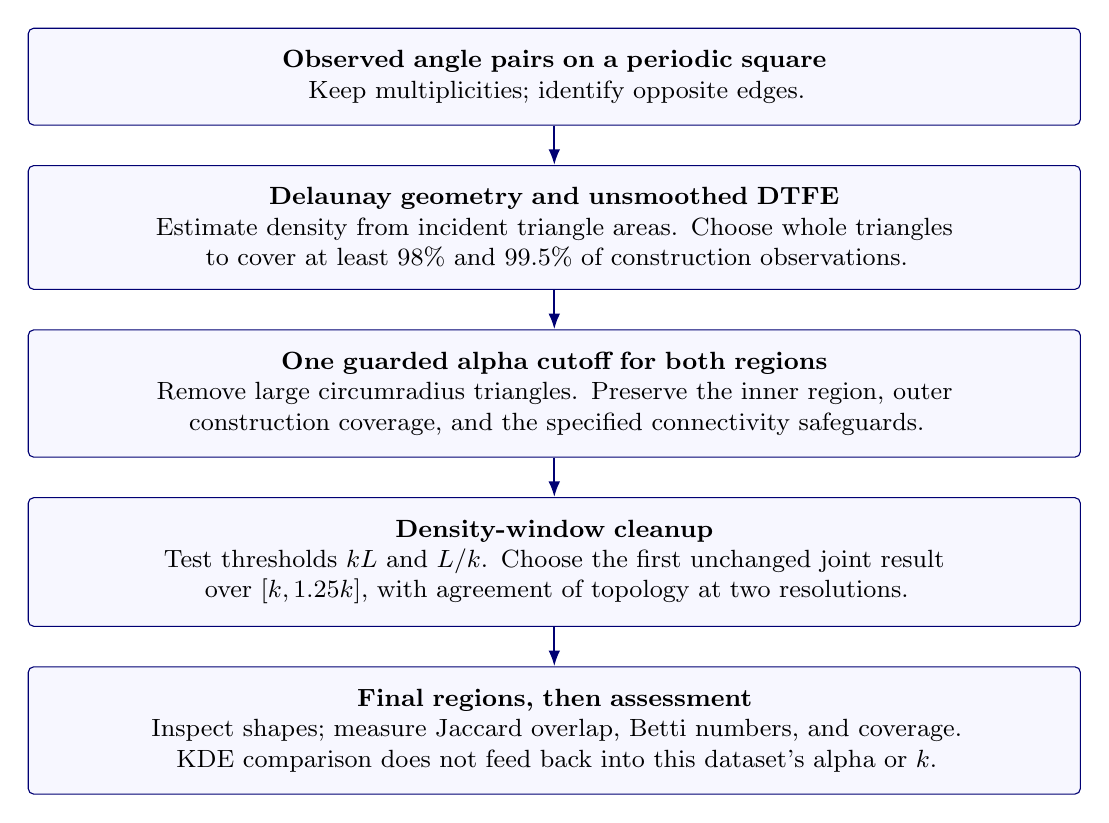
\begin{tikzpicture}[
  box/.style={draw=blue!45!black,rounded corners=2pt,fill=blue!3,
    text width=12.8cm,align=center,inner sep=8pt,font=\small},
  arrow/.style={-{Latex[length=2mm]},thick,draw=blue!45!black}]
\node[box] (data) {\textbf{Observed angle pairs on a periodic square}\\
  Keep multiplicities; identify opposite edges.};
\node[box,below=5mm of data] (density) {\textbf{Delaunay geometry and unsmoothed DTFE}\\
  Estimate density from incident triangle areas. Choose whole triangles\\
  to cover at least 98\% and 99.5\% of construction observations.};
\node[box,below=5mm of density] (alpha) {\textbf{One guarded alpha cutoff for both regions}\\
  Remove large circumradius triangles. Preserve the inner region, outer\\
  construction coverage, and the specified connectivity safeguards.};
\node[box,below=5mm of alpha] (epsilon) {\textbf{Density-window cleanup}\\
  Test thresholds $kL$ and $L/k$. Choose the first unchanged joint result\\
  over $[k,1.25k]$, with agreement of topology at two resolutions.};
\node[box,below=5mm of epsilon] (result) {\textbf{Final regions, then assessment}\\
  Inspect shapes; measure Jaccard overlap, Betti numbers, and coverage.\\
  KDE comparison does not feed back into this dataset's alpha or $k$.};
\foreach \a/\b in {data/density,density/alpha,alpha/epsilon,epsilon/result}
  \draw[arrow] (\a)--(\b);
\end{tikzpicture}
\caption{The adopted procedure. The density thresholds $L$ are fixed before
alpha and cleanup. The number 1.25 is the required span of stability, not the
cleanup ratio $k$. One rule is used for all six classes, with alpha and $k$
computed from each class's observations.}
\label{fig:flow}
\end{figure}

\section{The reference construction and the angular domain}
\label{sec:reference}

\subsection{How KDE turns observations into contours}

Kernel density estimation begins by placing a small, smooth mound around
each observation and adding the mounds. Where many observations are nearby,
their contributions accumulate. The width of a mound determines how much
neighboring observations influence one another. An adaptive KDE varies this
width with local sampling: dense regions receive finer detail, while sparse
regions are estimated over a wider neighborhood.

The Ramachandran procedure described by \citet{lovell2003} uses two passes
with compact radial cosine kernels. A first density estimate supplies the
local information used to choose the second-pass widths. The published
Top8000 generation recipe specifies periodic evaluation on a $2^\circ$ grid,
with a separate width setting for General and a common setting for the other
classes \citep{top8000recipe}. The final percentage convention ranks density
values evaluated at the construction observations. Thus a nominal 98\%
contour is tied to a fraction of those observations; it is not, merely by its
label, a guarantee about previously unseen proteins.

For comparison we use the distributed percentile grids themselves. They
store density ranks, rather than probability-density values. We interpolate
these scores periodically and bilinearly, and take scores at least $0.02$
and $0.005$ for our two chosen comparison levels, 98\% and 99.5\%. The latter
is a level selected for this study, not a claim about the standard MolProbity
allowed-region cutoff. The interpolation rule and these cutoffs completely
specify the reference regions used here. No refitting of the reference is
needed to draw the comparisons.

Our method uses construction counts too, but assigns those counts to a
different geometric family: unions of triangles. This keeps the purpose of
the percentage labels comparable while allowing the density estimator and
boundary representation to differ. It also makes an honest distinction
possible between achieving a construction target and subsequently measuring
agreement with a published region.

\subsection{A square whose opposite edges meet}

Both angles repeat every $360^\circ$. The natural domain is therefore
\[
  \Omega=(\R/360\Z)^2,
\]
shown as $[-180^\circ,180^\circ)^2$. A point near the right edge is close to
one near the left edge; a region that crosses an edge has not thereby split
into two. The same applies at the top and bottom. Distances use the nearest
periodic displacement in each coordinate, followed by the ordinary Euclidean
norm, with both coordinates measured in degrees.

The construction identifies equal periodic coordinates and records their
positive integer multiplicities $w_i$. Write $x_i$ for the resulting distinct
locations and $N=\sum_i w_i$ for the number of observations. Translated copies
of a location may be needed to construct triangles across an edge. They are
geometric copies only: their observations are counted once. This convention
is used throughout the density calculation, alpha selection, and topology
measurement.

\section{From Delaunay triangles to a density-based region}
\label{sec:dtfe}

\subsection{Estimating density from the space around an observation}

A Delaunay triangulation joins the locations into triangles whose open
circumdisks contain no other sample locations. A circumdisk is the disk
bounded by the circle through the three corners of a triangle. On our
periodic domain, the emptiness condition includes the translated sample
locations. The triangulation must cover the angular domain consistently,
including its seams. We use a fixed triangulation when a degenerate
configuration permits more than one choice.

The triangulation records local sampling scale without first choosing a
smoothing width. Nearby observations generally form small triangles; sparse
neighborhoods require larger ones. To turn this geometry into a density,
give each corner one third of every incident triangle's area. The total area
assigned to location $x_i$ is
\begin{equation}
 A_i=\frac13\sum_{\text{triangle corners at }i}\area(T),
 \qquad \rho_i=\frac{w_i}{A_i}.
 \label{eq:dtfe}
\end{equation}
All periodic corner incidences are included. We require $A_i>0$. In words,
the density is the number of observations at a location divided by the area
assigned to that location. This is the idea behind the Delaunay Tessellation
Field Estimator, or DTFE \citep{schaap2000}. Figure~\ref{fig:dtfe} illustrates
the assignment. The shaded thirds are an accounting device; the algorithm
does not need to construct those smaller polygons.

\begin{figure}[htbp]
\centering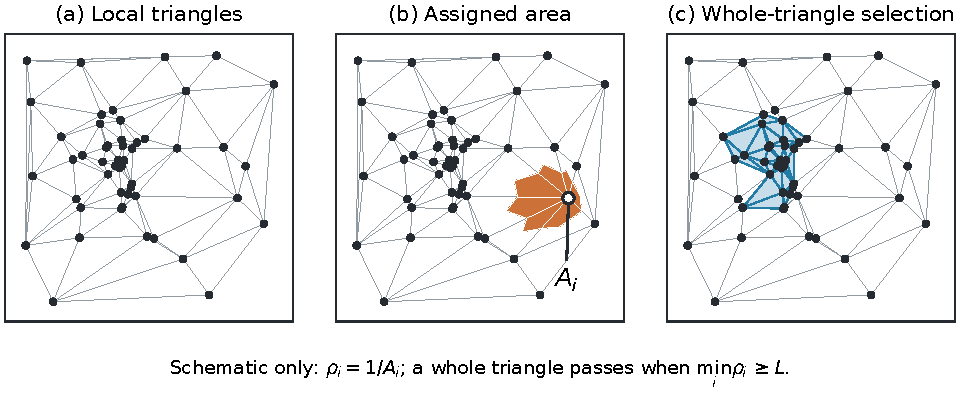
\includegraphics[width=\linewidth]{dtfe_schematic.pdf}
\caption{A schematic of the density construction. (a) The triangulation
adapts to the spacing of the observations. (b) The marked location receives
one third of each incident triangle, giving its assigned area $A_i$.
(c) A triangle is retained only when all three corner densities pass the
chosen threshold. These illustrative points are not a Top8000 subsample.}
\label{fig:dtfe}
\end{figure}

There is a useful accounting identity behind this estimate. Interpolate
the corner densities affinely inside every triangle, meaning by the unique
linear plane taking those three corner values. Call the resulting continuous
field $\rho(x)$. The average of an affine function over a triangle is the
average of its three corner values, so
\begin{equation}
 \int_\Omega\rho(x)\,dx
 =\sum_T\frac{\area(T)}3\sum_{i\in T}\rho_i
 =\sum_i A_i\rho_i=\sum_i w_i=N.
 \label{eq:mass}
\end{equation}
Consequently $\rho/N$ has probability-density units. Dividing all densities
and thresholds by $N$ changes no region in our method. No area floor or
smoothing correction enters~\eqref{eq:dtfe}.

\subsection{Why use whole triangles?}

The affine field explains the density estimate and its mass identity, but
our contours are built from whole triangles. Give a triangle the score
\begin{equation}
 g_T=\min_{i\in T}\rho_i.
 \label{eq:gate}
\end{equation}
At a threshold $L$, retain $T$ precisely when $g_T\geq L$. All its corners
then support its inclusion. This is a deliberately conservative way to use
the local density: a single high corner does not admit a thin wedge of an
otherwise weak triangle. The boundary follows existing edges, which gives
it an angular appearance and a clear relationship to the observations.

The minimum-corner score is a convenient selection score, not another
normalized density estimator. In particular, integrating this piecewise
constant score does not give the mass identity~\eqref{eq:mass}. We determine
the percentage labels by counting observations in the triangle union.

At this stage there is no alpha restriction. An observation at vertex $i$
belongs to the union if at least one incident triangle is selected. Its
inclusion height is therefore
\begin{equation}
 h_i(\infty)=\max_{T\ni i}g_T.
\end{equation}
For $q\in\{0.98,0.995\}$, sort these heights from largest to smallest and
accumulate their integer weights. Choose the highest threshold $L_q$ whose
inclusive count reaches $m_q=\lceil qN\rceil$. Include the entire tied group
at the threshold; record any resulting excess over $m_q$. The starting
region is
\begin{equation}
 S_q(\infty)=\bigcup_{g_T\geq L_q}T.
 \label{eq:baseline}
\end{equation}
Triangles are closed: their edges and corners belong to the region.
An observation incident to several selected triangles is still counted only
once, with its multiplicity. This convention also means that two triangles
meeting at a single corner are connected.

The 98\% region is contained in the 99.5\% region because
$L_{.98}\geq L_{.995}$. We refer to them as the inner and outer regions.
Their percentages are construction targets, achieved before the final
cleanup. Equation~\eqref{eq:baseline} does not establish coverage on new
observations, nor does it assert that the region contains $q$ of the
integrated density in~\eqref{eq:mass}.

\section{Alpha: removing sparse connections without sacrificing the core}
\label{sec:alpha}

\subsection{The geometric problem}

Passing a density threshold does not ensure that a triangle provides a
plausible connection. Its corners may lie in well-supported neighborhoods
while its interior spans a sparsely sampled gap. Whole-triangle selection
can then connect concentrations that should remain separate. CisPro gives
a concrete example in Figure~\ref{fig:cispro}.

Alpha shapes supply a geometric way to limit such triangles
\citep{edelsbrunner1983}. Let $R_T$ be the circumradius of $T$. For a chosen
radius $a$, we retain only triangles with $R_T\leq a$:
\begin{equation}
 S_q(a)=\bigcup_{\substack{g_T\geq L_q\\R_T\leq a}}T.
 \label{eq:alpha}
\end{equation}
Here alpha is the radius itself, measured in degrees, rather than its
square. We use the filled triangle part of this construction; isolated
edges or vertices are not added as separate contour regions. A large
circumradius indicates an empty disk at a large angular scale. It can
therefore detect both a long span and an unusually thin triangle. The
cutoff addresses geometric support, not density averaging.

\begin{figure}[htbp]
\centering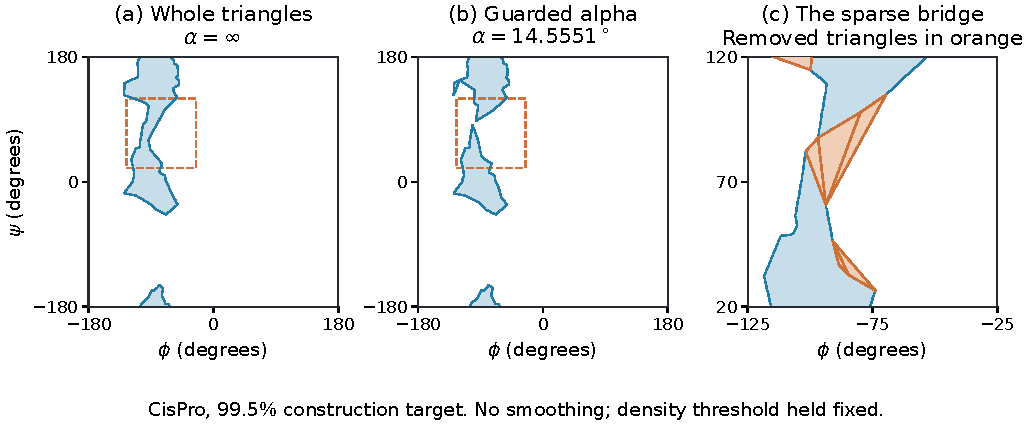
\includegraphics[width=\linewidth]{cispro_alpha.pdf}
\caption{What alpha changes in CisPro at the 99.5\% target. (a) Whole
triangles at infinite alpha contain a sparse connection. (b) The common
guarded rule selects $a=14.5551^\circ$ and removes it. (c) The boxed area
is enlarged; orange shows the removed triangles in that neighborhood.
Eleven triangles are removed in total, reducing the exact outer area by
11.53\%. The inner triangles and the required 3,506 outer observations
remain. These panels show our geometry alone, without a KDE overlay.}
\label{fig:cispro}
\end{figure}

\subsection{Choosing one radius by explicit safeguards}

A very small radius could destroy useful regions along with an unwanted
bridge. We therefore select alpha subject to four safeguards, using the
same radius for both levels and holding $L_{.98}$ and $L_{.995}$ fixed.
Each safeguard has a particular purpose:
\begin{enumerate}
\item \textbf{Preserve the complete inner region.} Every triangle in
$S_{.98}(\infty)$ must remain. The outer region may be pared back, but not
by sacrificing the previously selected inner geometry.
\item \textbf{Retain outer construction coverage.} The remaining outer
region must still contain at least $\lceil .995N\rceil$ weighted
observations. Any removal of observations is limited to the available
rounding or tie excess.
\item \textbf{Do not create a new isolated excluded region.} Every connected
component of the candidate's open complement must contain a triangle from
the original outer complement. In ordinary planar language, this prevents
excising a new hole from the interior. The condition tracks where excluded
space came from, rather than merely comparing total component counts.
\item \textbf{Allow only supported splits.} If a connected component of
the original outer region splits into two or more surviving pieces, every
piece must contain an unchanged inner triangle. Thus a split can separate
supported concentrations, but cannot shed new pieces lacking an inner core.
An already coreless outer component may remain or shrink; the rule does
not require it to disappear.
\end{enumerate}

Connectivity is computed on the periodic triangle geometry. Selected closed
triangles connect through shared corners as well as edges. The open
complement connects through shared edges of unselected triangles, not by
passing through a selected corner. These different conventions follow from
the distinction between a closed region and its open complement.

Among candidates passing all four conditions, choose the one with smallest
outer area, summing triangle areas before any rasterization. Since the inner
region is fixed, this is also the minimizer of the sum of inner and outer
areas. Only the active outer-triangle circumradius values and infinity need
be examined: between them the selected triangle sets do not change. All
triangles tied at a radius are included. If evaluated candidates give
identical triangle sets, prefer the least restrictive of them, with infinity
preferred when it gives the same geometry. Infinity always passes, so the
method never has to impose a damaging finite cutoff.

This rule does not request two components for CisPro or specify a desired
number for any other class. It also does not force different inner
components to become different outer components: a supported outer bridge
can remain, as in TransPro. Its objective is to remove unnecessary area
while respecting the declared structural commitments.

\begin{proposition}[Construction thresholds remain calibrated]
If a selected alpha retains the required construction count at $L_q$, then
$L_q$ remains the highest feasible density threshold for that alpha.
\end{proposition}
\begin{proof}
Every threshold above $L_q$ already covered too few observations at infinite
alpha. Imposing a finite alpha only removes triangles, so cannot increase
that count. The selected alpha still meets the target at $L_q$ itself.
\end{proof}

Nesting also survives because the same radius is applied to both ordered
thresholds. These are properties of the alpha stage. They do not promise
that every small island should be retained indefinitely, or that the final
cleanup will leave construction coverage unchanged.

\section{A density window for islands and holes}
\label{sec:cleanup}

\subsection{What alpha leaves behind}

Alpha can remove a sparse connection, but it need not remove a tiny island
made entirely of small triangles. Raw local density estimates can contain
many such features, as well as small low-density pockets inside larger
regions. Their total area may be modest while their visual and topological
effect is substantial. The first column of Figure~\ref{fig:cleanup} shows
this distinction: General's broad regions are recognizable, but hundreds
of components remain.

Our final step asks whether these features are substantial relative to
their own contour's density threshold. An island should contain a higher
density core if it is to survive stronger cleanup. A hole may be filled
when it is only a shallow depression, provided filling it does not undo
alpha or alter the periodic exterior. This changes entire features while
preserving the edge geometry of surviving boundaries; it does not move
observations or apply a smoothing kernel.

\begin{figure}[htbp]
\centering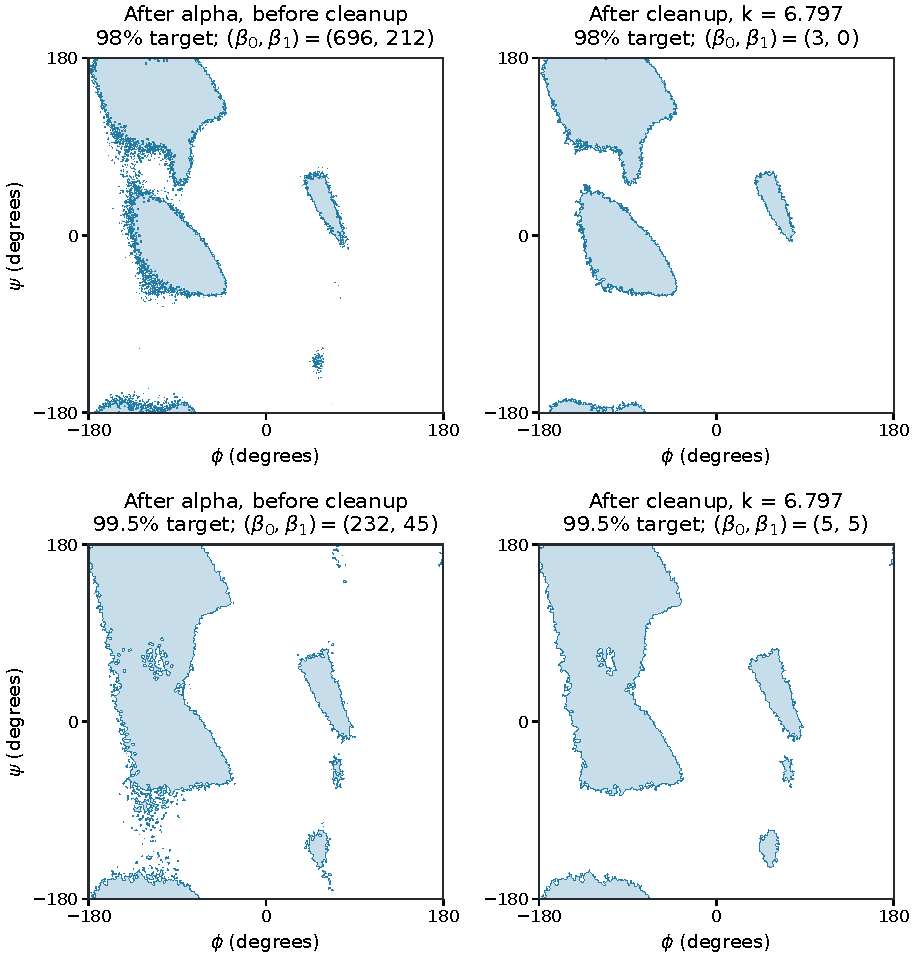
\includegraphics[width=.93\linewidth]{general_cleanup.pdf}
\caption{General before and after the selected density-window cleanup.
The levels are shown in separate rows to keep their boundaries readable.
The 98\% component count falls from 696 to 3 and the 99.5\% count from 232
to 5 on the $1536\times1536$ grid. The surviving boundaries remain jagged.
Here $(\beta_0,\beta_1)$ denotes components and independent loops; the
periodic interpretation is explained in the text. No KDE is drawn in this
method illustration.}
\label{fig:cleanup}
\end{figure}

\subsection{Defining the sampled field and its topology}

Let $D_a$ be the union of all alpha-eligible triangles, including those
below the two contour thresholds. Within this domain, use the score
\begin{equation}
 F_a(x)=\max\{g_T:x\in T,\ R_T\leq a\},
 \label{eq:field}
\end{equation}
and set it to zero where no eligible triangle contains $x$. The maximum
specifies membership consistently at shared closed edges and corners.
Thus $S_q(a)=\{x\in D_a:F_a(x)\geq L_q\}$.

The implemented cleanup uses a square grid. Divide each angular axis into
$n$ equal intervals, producing $n^2$ little squares, which we call pixels
or grid squares. Sample~\eqref{eq:field} and alpha eligibility at each
square's center. A foreground square is one whose center belongs to
$S_q(a)$; all other squares form the background. The resulting Boolean
array is its mask. We use $n=768$ and $1536$, with widths $0.46875^\circ$
and $0.234375^\circ$, respectively, and the same origin at $-180^\circ$.

Foreground squares connect along either an edge or a corner (eight
neighbors); background squares connect along edges (four neighbors).
Opposite grid edges are identified. This gives the topology of a union of
closed foreground squares. It approximates the triangle region, but is not
a certificate of that region's exact topology.

We record two Betti numbers. The number $\beta_0$ counts connected pieces.
The number $\beta_1$ counts independent loops: closed paths that cannot be
contracted within the region. For ordinary bounded patches these often
correspond to holes. On a periodic square, a path may also wind around an
angular direction, so ``loop'' and ``interior hole'' are not synonymous.
In particular, opposite-edge fragments must not be counted separately just
because the display cuts through them.

\subsection{The cleanup operation at a fixed strength}

Write $L$ for either $L_q$ and let $k\geq1$. The two comparison thresholds
are
\begin{equation}
 L_{\mathrm{high}}=kL,\qquad L_{\mathrm{low}}=L/k.
 \label{eq:window}
\end{equation}
They form a symmetric interval on a logarithmic density scale:
$[\log L-\log k,\log L+\log k]$. This is the precise meaning of the
``epsilon jiggle'' here. The level is varied; coordinates are never
jittered. Equivalently, $\varepsilon=\log k$ is the half-width in log
density. It is not an additive tolerance in degrees.

For each starting foreground component, find the largest sampled score
within it, its \emph{peak}. Delete the entire component only if this peak
is strictly below $kL$. Equality retains it. A surviving island therefore
contains a core that reaches the higher threshold. This criterion measures
relative density support, not island area.

Next recompute the background components \emph{after these deletions}.
Removing an island or a weak ring can join background pieces that were
previously separate. Using the old background labels could fill the center
of a deleted ring as an isolated new island, defeating the operation's
purpose. For each recomputed background component, find its smallest score,
its \emph{pit}. Fill the component if its pit is at least $L/k$, except
when any of the following applies:
\begin{enumerate}
\item it winds around either periodic angular direction;
\item it is tied for largest background area;
\item it contains any alpha-ineligible grid square.
\end{enumerate}
The first two exclusions protect exterior-like background; on a torus
there is no unique unbounded exterior to select automatically. All
largest-area ties are protected so array traversal cannot decide the
answer. The third exclusion protects the \emph{entire} background
component containing an alpha-excluded square. In particular, cleanup
cannot fill an eligible portion of a gap in a way that restores a
connection removed by alpha.

\begin{proposition}[A bounded density window]
On the sampled grid, the cleaned region $C_q(k)$ satisfies
\begin{equation}
 D_a\cap\{F_a\geq kL_q\}\ \subseteq\ C_q(k)\
 \subseteq\ D_a\cap\{F_a\geq L_q/k\}.
 \label{eq:sandwich}
\end{equation}
At $k=1$ the cleanup leaves the starting mask unchanged.
\end{proposition}
\begin{proof}
A square reaching $kL_q$ lies in a starting component whose peak reaches
that threshold, so its component is retained. Any retained starting square
has score at least $L_q\geq L_q/k$. Any filled square belongs to an
alpha-eligible component whose minimum score is at least $L_q/k$.
For $k=1$, no starting component fails its own level and every unprotected
background component contains a square below it, so neither operation
changes the mask.
\end{proof}

This gives an explicit spatial and density constraint, not a guarantee
that each removed feature was noise. A large but low-peaked island may
disappear before a tiny but high-peaked one. Nor can this operation sever
a bridge within a retained component: bridge removal belongs to alpha.
Because deletion and filling have different effects, the cleaned regions
are not assumed to vary monotonically with $k$, or to remain nested across
the two target levels without checking.

The use of two nearby density levels is related to the approach of
\citet{bobrowski2017}, who study the topology surviving the inclusion from
a higher-level set into a lower-level set. An induced homology map records which components and loops survive
that inclusion; its image is their output, rather than a unique cleaned contour. Our whole-component
deletion and protected hole filling are a separately specified geometric
rule. Raw DTFE, alpha restriction, this multiplicative window, and the
periodic raster do not inherit their kernel-estimation consistency theorem.
Equation~\eqref{eq:sandwich} is a property of our operation; it must not be
substituted for that statistical theorem.

A computational precedent for simplifying unsmoothed DTFE topology is
DisPerSE \citep{sousbie2011}. It constructs a discrete Morse complex from
Delaunay-based density estimates and cancels persistence pairs below a
significance threshold calibrated on Poisson samples. A pair's density
ratio measures its contrast; taking logarithms converts this ratio into
an additive difference. Thus DTFE followed by topological simplification,
including relative density comparisons, is established prior work.
Our operation shares the aim of suppressing weak density features without
convolution, but uses the peaks and pits of components at a fixed contour
level, with alpha and periodic-background protections. It neither computes
persistence pairs nor cancels critical simplices. In particular, $k$
compares each peak or pit with $L$; it is not a persistence-pair ratio.
The plateau rule below selects $k$ by output stability, not a Poisson-noise
significance calibration, and does not inherit DisPerSE's significance
interpretation.

\subsection{Choose the first stable window, then stop}
\label{sec:span}

The ratio $k$ controls how aggressively we simplify. Choosing it separately
by eye for every class would leave the procedure underspecified. We instead
examine the full set of changes over the declared range $1\leq k\leq64$.
On a finite grid, only finitely many comparisons can change: a peak can
cross $kL$, or a pit can cross $L/k$. Between actual changes the complete
output mask is constant. We call such an interval a \emph{plateau}.

Run this event calculation for both target levels on both grids, and merge
the four lists of change points. A joint plateau means that each of the
four masks is unchanged throughout that interval. We require complete
region identity, not merely unchanged Betti numbers: one island could
vanish while another appears, leaving the counts unchanged but the shape
different.

The adopted stopping rule selects the first joint plateau with left onset
$k$ that satisfies all of the following:
\begin{enumerate}
\item it contains the whole closed interval $[k,1.25k]$;
\item $\beta_0$ and $\beta_1$ agree between resolutions at each target;
\item both regions are nonempty on both grids;
\item the inner mask is contained in the outer mask on each grid.
\end{enumerate}
Return that $k$ for both target levels of the class. Different classes may
return different ratios, but use exactly the same test. If the next actual
change is at $b$, the first condition requires $1.25k<b$, because including
$b$ would include a changed region. For a final interval only observed
through 64, $1.25k\leq64$ is sufficient; it makes no claim beyond the
observed range. If no interval qualifies, report the selection unresolved.
Do not substitute a default strength or silently widen the search.

Strict inequalities require care at event boundaries. For example, a peak
equal to $kL$ is retained and disappears just above the limiting ratio.
The implementation enumerates the actual floating-point transition
onsets, taking the first representable value at which the predicate
changes. These saved values, rather than rounded display values, define
the returned left endpoint. This operational convention makes the first
onset unambiguous even when the corresponding real-number interval would
be open on the left.

\begin{figure}[htbp]
\centering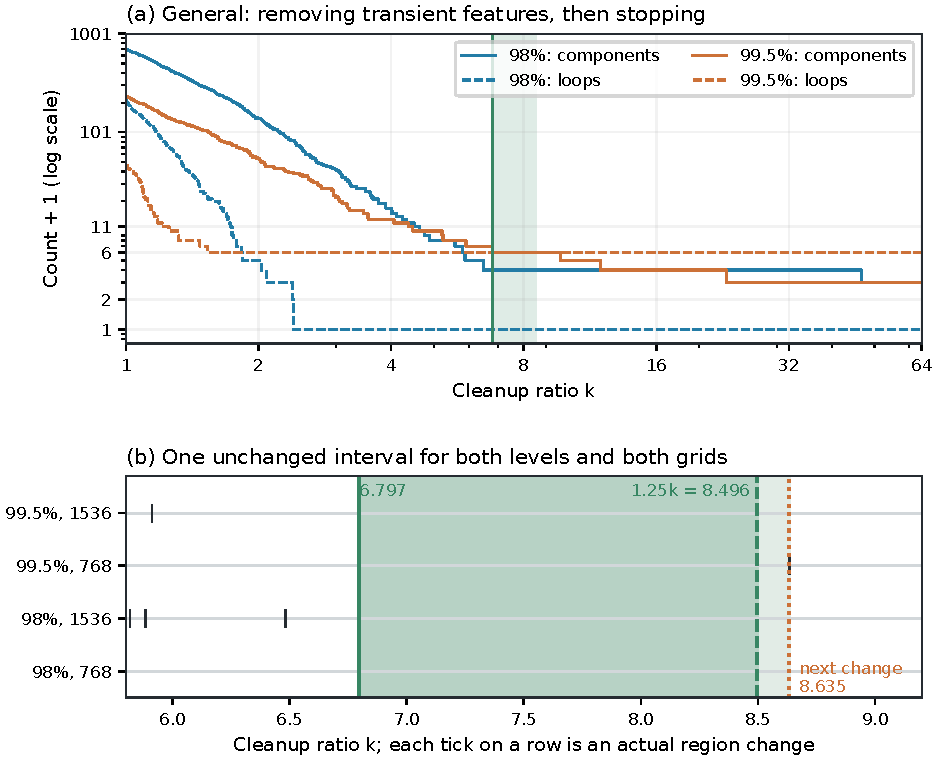
\includegraphics[width=\linewidth]{general_stability.pdf}
\caption{Selecting the General cleanup strength without a KDE target.
(a) Components and loops change as $k$ increases; one is added to the counts
so zeros can be shown on a logarithmic axis. (b) Each tick records a change
of an entire mask. The selected joint plateau begins at $k=6.796947\ldots$
and lasts until $8.634671\ldots$. The required interval ends earlier, at
$1.25k=8.496184\ldots$, and lies entirely inside it. The displayed Betti
curves illustrate simplification; the selector checks mask identity and
the additional conditions in Section~\ref{sec:span}.}
\label{fig:stability}
\end{figure}

\subsection{Why a factor of 1.25?}

The stopping question is local: has a modest further increase in cleanup
stopped changing the answer? Requiring a 25\% relative increase gives this
question a fixed, testable meaning. It is dimensionless, works at $k=1$ as
well as at larger ratios, and, in exact arithmetic, is unchanged by multiplying all density
values and thresholds by a common constant. It avoids comparing an
absolute density tolerance across classes with very different populations.

Stopping at the \emph{first} qualifying interval is as important as its
width. A stronger cleanup can eventually remove a substantial island and
produce another, longer plateau. That does not invalidate the earlier
local plateau. If every later simplification were used as a reason to
demand more stability, the rule would tend toward increasingly stripped
regions rather than a reproducible stopping point.

Figure~\ref{fig:features} shows the tradeoff directly. The General outer
island near $(73^\circ,-51^\circ)$ survives the selected $k$, but disappears
under stronger cleanup. The small inner island near
$(53^\circ,-127^\circ)$ disappears earlier, before the selected interval.
The method therefore retains substantial structure without pretending to
distinguish every meaningful island from every fluctuation.

The numerical factor 1.25 is an empirical convention for this protocol
version, not a uniquely derived constant or a theorem of optimality. It
was adopted during Top8000 development with access to the reference
comparisons. Its independent justification is the stated local robustness
requirement and the preference to stop before further unnecessary feature
loss. Once fixed, the per-dataset selector uses only our density field,
geometry, and resolution checks. A future application needs no KDE to
compute alpha or $k$; a future reference comparison should assess the
result without changing this version's rule. The endpoint 64 and the two
grid sizes are likewise declared numerical settings, not universal laws.

\begin{figure}[htbp]
\centering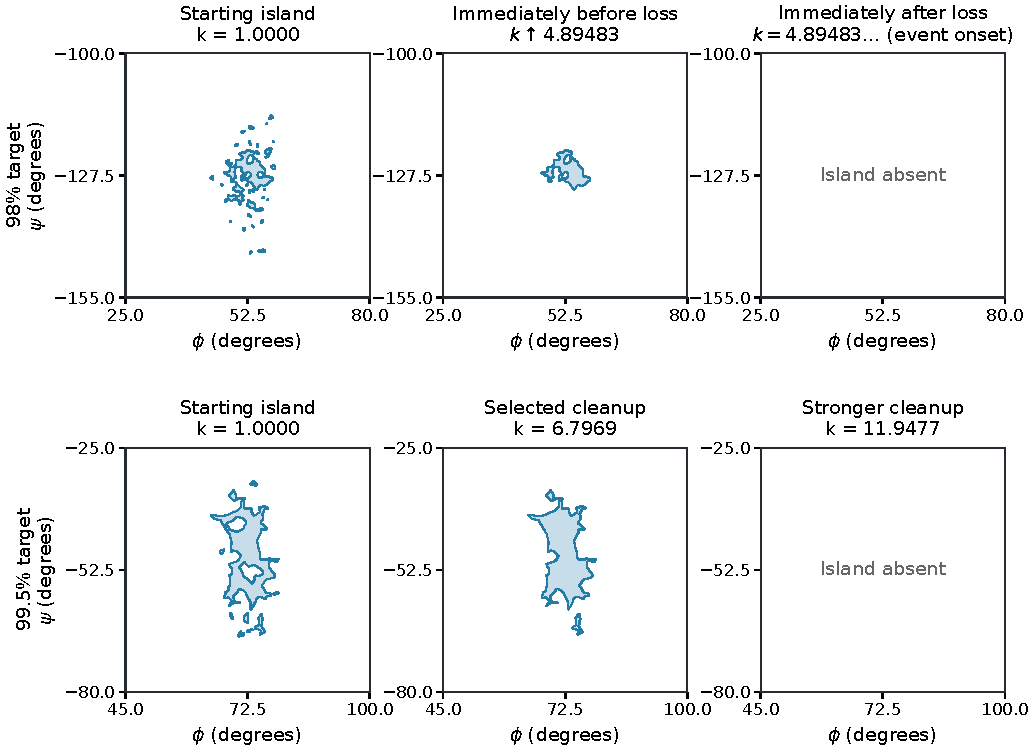
\includegraphics[width=\linewidth]{general_feature_fates.pdf}
\caption{Features have identifiable disappearance thresholds. The top
row follows General's small 98\% island through its loss at the event
$k=4.894829\ldots$. The bottom row follows a different, 99.5\% island:
it remains at the selected $k=6.796947\ldots$ and disappears at
$11.947717\ldots$. Coordinates identify the same neighborhood across
each row. These are cropped computed masks, with no KDE input or overlay.
Larger $k$ can remove a recognizable island, which explains the decision
to stop at the first qualifying plateau.}
\label{fig:features}
\end{figure}

\FloatBarrier
\section{What the six-class results establish}
\label{sec:results}

\subsection{Parameters produced by the common rule}

Table~\ref{tab:parameters} records the full available two-angle construction
populations and the computed parameters. No reduced fitting sample is used
for these figures. The six numerical alpha and $k$ values are outputs of
the rule, not class constants to copy onto a new dataset. In particular,
the larger CisPro radius is not a special instruction for proline.

\begin{table}[htbp]
\centering
\begin{tabular}{lrrr}
\toprule
Class & Observations $N$ & Alpha radius $(^\circ)$ & Cleanup $k$\\
\midrule
\tableinput tables/parameters.tex 
\bottomrule
\end{tabular}
\caption{Computed outputs for the six Top8000 construction populations.
The stability span is 1.25 for every row. Values are rounded for reading;
the accompanying numerical record retains full precision for computation.}
\label{tab:parameters}
\end{table}

All six inner triangle regions survive alpha unchanged. Only CisPro's
outer component splits: its exact triangle topology changes from one
component to two, with both pieces retaining inner triangles. Its outer
area falls from $9884.44$ to $8744.91$ square degrees while retaining the
required 3,506 observations. For each of the other five classes, less than
0.67\% of outer area is removed and outer connectivity is unchanged.
These results show why a common guard is preferable to a rule that insists
every class should have its outer connections broken.

After alpha, the first stable choice for CisPro is $k=1$. Its cleanup is
therefore the identity. This is a useful outcome: the same protocol may
decide that a class needs no additional simplification. In the denser
classes the window removes many small features, while leaving the
surviving boundaries at their original angular locations.

\subsection{Agreement in area and visible shape}

For a final region $C$ and reference region $K$, the Jaccard score is
\begin{equation}
 J(C,K)=\frac{\area(C\cap K)}{\area(C\cup K)}.
 \label{eq:jaccard}
\end{equation}
It equals one for identical regions and zero for disjoint regions of
positive area. Our reported values count squares on the common
$1536\times1536$ grid; thus they are raster approximations to area overlap.
This is an area measure, not a percentage of observations classified alike.

Figures~\ref{fig:kde98} and~\ref{fig:kde995} show the final regions with the
published boundaries. The principal concentrations occupy similar places
and have recognizable corresponding outlines. General's main regions and
the broad IleVal and PrePro shapes are recovered; TransPro retains its
outer connection; CisPro's unwanted bridge has been removed. The
construction consequently meets the central feasibility goal: Delaunay
density and guarded alpha, followed by a reproducible cleanup, can produce
readable Ramachandran regions resembling the academic reference without
using that reference in per-dataset parameter selection.

The degree of resemblance must still be read quantitatively.
Table~\ref{tab:agreement} gives final Jaccard values from 0.712 to 0.880.
Cleanup improves overlap for the ten contours it changes and leaves the
two CisPro values unchanged. Alpha itself is not an overlap optimizer:
it improves CisPro's outer score from 0.683 to 0.712 while decreasing the
other five outer scores by at most 0.0024. Those small costs accompany its
explicit geometric objective, rather than a hidden KDE-based choice.

The triangular representation explains much of the finer jaggedness.
The raster adds a smaller staircase effect. It does not follow that all
disagreement is harmless roughness: some broad boundary offsets and missing
islands are real differences between the constructions. Visual comparison
is needed precisely to distinguish these cases.

\begin{figure}[htbp]
\centering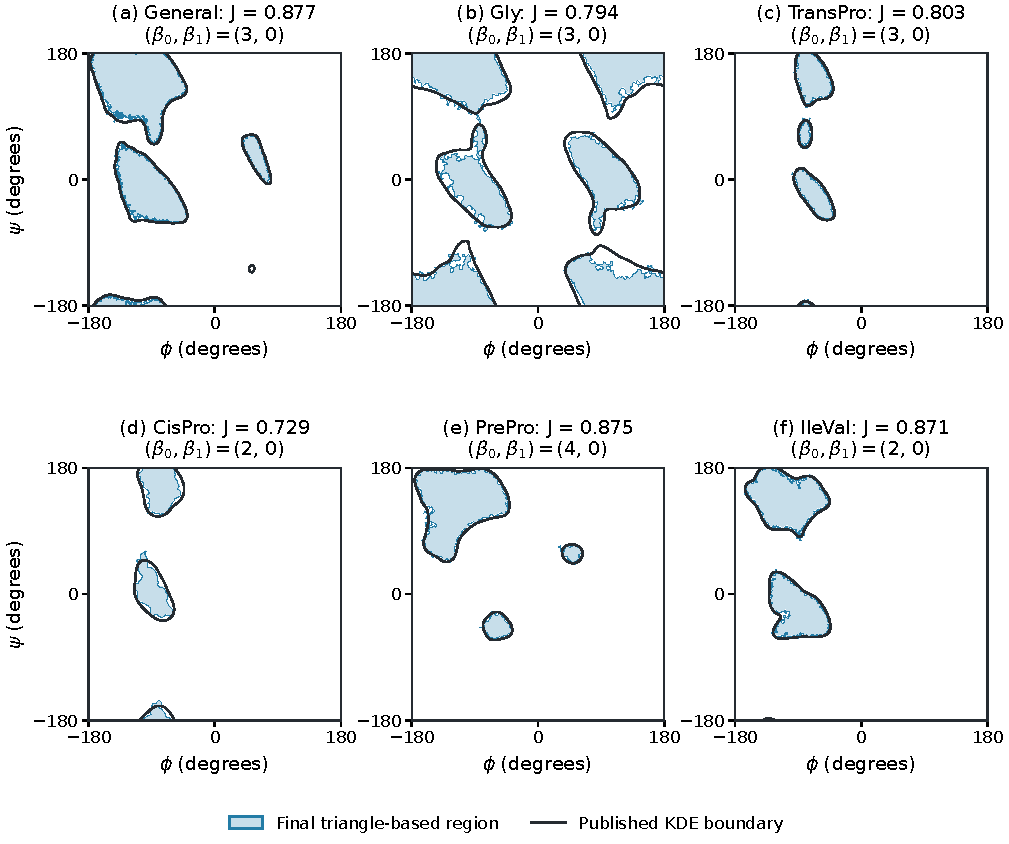
\includegraphics[width=\linewidth]{kde_comparison_980.pdf}
\caption{Final regions at the 98\% construction target. Blue fill and
blue edges show our adopted DTFE--alpha--cleanup result; black lines show
the published Top8000 percentile-grid boundary. Each panel reports its
Jaccard score and our raster $(\beta_0,\beta_1)$. The same periodic angular
domain and display conventions are used in every panel. General's small
lower-right reference island is absent from the final region; PrePro
retains an additional component. The label identifies the pre-cleanup
construction target, not an exact final raster-coverage statement.}
\label{fig:kde98}
\end{figure}

\begin{figure}[htbp]
\centering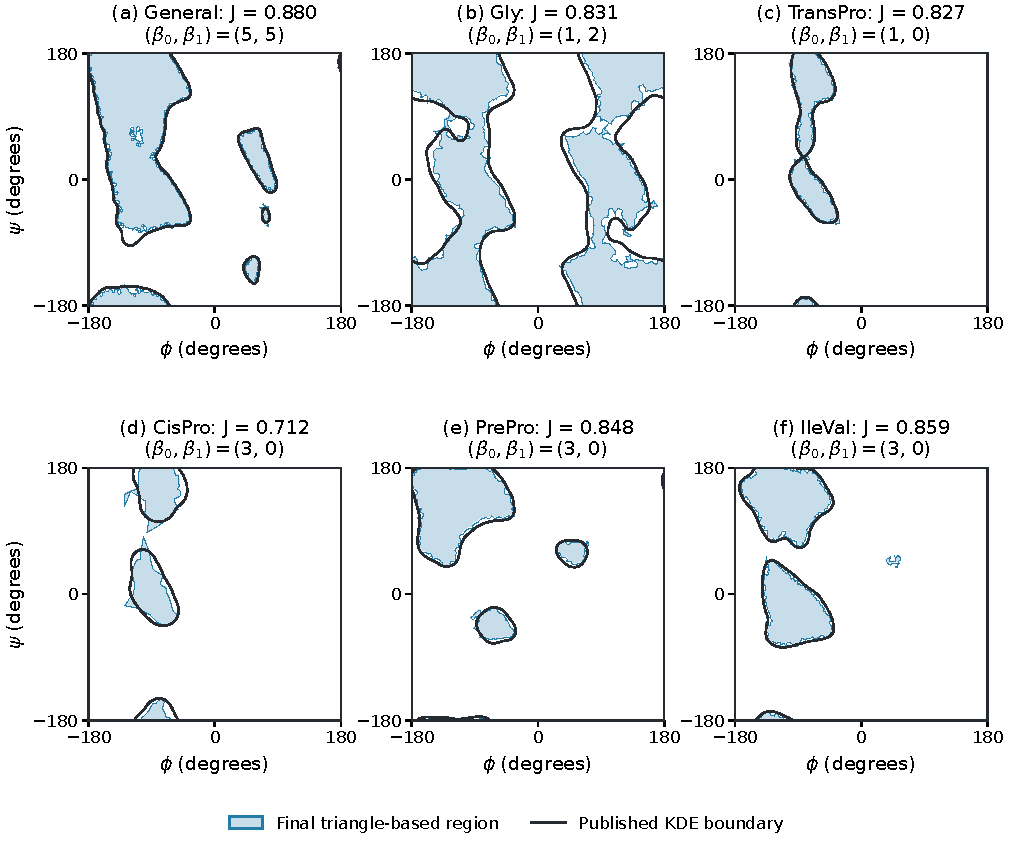
\includegraphics[width=\linewidth]{kde_comparison_995.pdf}
\caption{Final regions at the 99.5\% construction target, using the same
conventions as Figure~\ref{fig:kde98}. The dominant shapes remain
recognizable, with jagged triangle-derived boundaries. General retains
both tracked outer islands, but also retains protected small loops.
CisPro has no central bridge; the difference between its exact triangle
connectivity and raster connectivity is discussed in the text. IleVal
retains a small additional outer component. A reference boundary crossing
opposite plot edges remains connected on the angular domain.}
\label{fig:kde995}
\end{figure}

\begin{table}[htbp]
\centering\small
\setlength{\tabcolsep}{5pt}
\begin{tabular}{lrccccc}
\toprule
& Target & \multicolumn{2}{c}{Jaccard} & \multicolumn{3}{c}{$(\beta_0,\beta_1)$}\\
\cmidrule(lr){3-4}\cmidrule(lr){5-7}
Class & (\%) & Alpha & Final & Alpha & Final & KDE\\
\midrule
\tableinput tables/agreement.tex 
\bottomrule
\end{tabular}
\caption{Area agreement and topology before and after cleanup, measured
on the same $1536\times1536$ grid. ``Alpha'' means the guarded alpha result
before cleanup. Seven of twelve final Betti pairs match the reference.
Counts supplement the overlays: they do not identify the locations,
areas, or biological significance of the features.}
\label{tab:agreement}
\end{table}

\subsection{Topology: substantial simplification, with specific residual differences}

The reduction in fragmentation is substantial. For General, the two
component counts fall from 696 and 232 to 3 and 5. The selected final
Betti pairs agree between the two tested resolutions for every class and
level. The inner and outer masks are nested at both resolutions. Seven
of the twelve pairs also agree with the reference.

The remaining differences are localized enough to describe. General loses
its small inner island, retains five outer components instead of four,
and has five outer loops rather than zero. These five loops enclose
background connected to alpha-ineligible squares, so the cleanup's own
protection rule deliberately prevents filling them. PrePro retains an
extra inner component, and IleVal an extra outer component. CisPro has
three outer raster components while the exact selected triangle union has
two: a sufficiently narrow contact can disappear when membership is
sampled at grid centers. Agreement of the two tested raster counts does
not certify the exact contact.

These qualifications matter, but they do not negate the recovery of the
principal regions. A Betti number gives the same unit weight to a tiny
fragment and a large conformational region; Jaccard can almost ignore a
very thin bridge. Their combination with the overlays gives a more useful
assessment than optimizing either quantity in isolation. In particular,
we do not claim that matching a Betti pair proves matching topology in
location or shape, or that a high overlap score excuses a wrong connection.

\subsection{What happens to the percentage labels?}

The triangle region after alpha meets its exact construction target.
Cleanup then deletes islands and fills holes at the fixed $L_q$, so it can
lower or raise coverage. We measure this change without recalibrating the
threshold. The final labels therefore name the construction targets from
which the regions were obtained.

There is also a separate numerical effect. The construction counts
observations in closed triangles, whereas the cleanup mask classifies an
observation by the grid square containing it. A triangle vertex can be
inside the exact region while that square's center is outside. For
example, CisPro's outer triangle region contains $3506/3523=99.517\%$ of
its observations, while its raster coverage is 98.325\%, even at $k=1$.
This discrepancy is from representation, not an unreported cleanup loss.

Using the same raster convention before and after cleanup isolates the
cleanup effect: across the twelve contours the change is between
$-0.2035$ and $+0.0706$ percentage points. For General the two changes are
$-0.0592$ and $-0.0421$ percentage points. These changes are small in
population fraction but do not justify claiming exact final coverage.
The numerical record accompanying the paper separates exact starting
counts from the two raster counts.

\FloatBarrier
\section{A reproducible procedure and its present scope}
\label{sec:scope}

\subsection{What is fixed, and what is learned from a new input?}

The protocol fixes the two target fractions, the minimum-corner triangle
rule, the four alpha guards, the cleanup operation, the two grids, the
search interval, and the 1.25 stability span. Given a new class of angular
observations, it computes the Delaunay geometry, the local densities, the
two calibrated thresholds, a shared alpha, and a shared cleanup ratio.
It can return an unresolved cleanup selection rather than force an answer.
This is the sense in which the method stands on its own: the computation
does not require a reference contour, a target Betti count, or manually
chosen island locations.

Its components have established precedents: DTFE estimates local density
from triangulation geometry, alpha shapes constrain empty spatial scales,
and density-level comparisons motivate examining the robustness of
features. The contribution here is their explicit combination for these
angular contour regions, with the interaction between construction
coverage, geometric guards, and cleanup spelled out. The application does
not require a claim that each ingredient is new.

The implementation records periodic geometry checks, tied observations,
calibrated counts, alpha candidates, and complete cleanup change events.
For the current data, the periodic mesh exports verify coverage of the
angular domain, paired edges, local vertex neighborhoods, and the required
empty-circumdisk conditions. The grid fields use that geometry without
smoothing. The selection records are written before the reference
assessment. All figures here were regenerated from the adopted saved masks,
whose hashes and twelve reported Jaccard values were checked by the
accompanying rendering script. The source bundle contains the figure
manifest, full-precision numerical tables, and this document's build recipe.

Computationally, both parameter searches are finite event searches.
Two-dimensional periodic triangulations have a number of triangles
proportional to their number of vertices; the alpha implementation can
skip radii already ruled out by inner preservation or outer coverage.
The cleanup can reuse component information and evaluate only actual
comparison changes. This is more informative than repeatedly choosing
arbitrary trial ratios. It does not by itself establish an end-to-end
speed or memory advantage over the academic KDE implementation. The
adopted stages have been run on the available six-class inputs; packaging
the same stages as a portable new-data interface remains an implementation
task, not evidence already supplied by these figures.

\subsection{What remains to be established}

Top8000 supports feasibility and development of the recipe. It is not an
independent validation population after the protocol choices were made.
Our supplied construction observations and the distributed reference also
need not be identical preparations; notably the published Gly reference
is symmetrized, while our fitted observations are not mirrored. Their
agreement should be interpreted as agreement of the resulting regional
descriptions, rather than exact reconstruction of the reference's input
pipeline.

A prospective Top2018 application should apply this fixed recipe first
and compare contours afterward. To interpret coverage on genuinely new
observations, overlap or relatedness between the source populations must
also be controlled. Within the present data, further numerical work should
test boundary convergence and shifted grid origins, rather than treating
agreement of two Betti pairs as full convergence. Resampling would address
a different question again: whether a feature survives changes to the
observations, not merely changes to $k$.

The intended next coordinate is the side-chain angle $\chi_1$, with
possible later $\chi_2$ and further $\chi$ angles. All remain periodic.
The DTFE accounting extends naturally: a $d$-dimensional simplex shares
its volume among $d+1$ corners, yielding the analogue of
\eqref{eq:mass}. Delaunay circumradii and nested construction thresholds
also have higher-dimensional counterparts. The planar cleanup and its
topology safeguards, however, require additional design for three-dimensional
tunnels and cavities, and regular grids grow rapidly with dimension.
Neither higher-dimensional accuracy nor superior tractability follows
from the two-dimensional result. Building and evaluating the
$(\phi,\psi,\chi_1)$ extension remains a research objective.

The present conclusion is correspondingly concrete. The three-stage
construction produces recognizable, quantitatively similar Top8000
regions with intentionally angular boundaries. It resolves the targeted
CisPro connection and most visible fragmentation using the same rules
across classes. The remaining islands, protected loops, raster contacts,
and coverage qualifications are part of the measured result. They define
where the procedure is already useful and where a stronger claim of
replacement for the reference still needs evidence.

\section*{Data and reproducibility}

The reference grids are attributed to the Richardson Laboratory and
distributed under CC BY 4.0. We use the pinned Top8000 reference snapshot
in the bibliography; the plotted reference boundary is derived by the
interpolation and cutoffs in Section~\ref{sec:reference}. Our newly drawn
blue regions use the recorded full six-class construction populations.
The numerical procedure is versioned as \protocol. The accompanying
\texttt{README.md} maps each figure and table to its input records and
provides commands to rebuild this exposition.

{\small
\setlength{\bibsep}{5pt}
\bibliographystyle{unsrtnat}
\bibliography{references}
}
\end{document}
